\documentclass[nojss]{jss}

%% -- LaTeX packages and custom commands ---------------------------------------

%% recommended packages
\usepackage{orcidlink,thumbpdf,lmodern}

%% new custom commands
\newcommand{\class}[1]{`\code{#1}'}
\newcommand{\fct}[1]{\code{#1()}}

%% For Sweave-based articles about R packages:
%% need no \usepackage{Sweave}



%% -- Article metainformation (author, title, ...) -----------------------------

%% - \author{} with primary affiliation (and optionally ORCID link)
%% - \Plainauthor{} without affiliations
%% - Separate authors by \And or \AND (in \author) or by comma (in \Plainauthor).
%% - \AND starts a new line, \And does not.
\author{Alexander Pate~\orcidlink{0000-0002-0849-3458}\\University of Manchester
  \And Glen P. Martin\\University of Manchester}
\Plainauthor{Alexander Pate, Glen P. Martin}

%% - \title{} in title case
%% - \Plaintitle{} without LaTeX markup (if any)
%% - \Shorttitle{} with LaTeX markup (if any), used as running title
\title{calibmsm: An \proglang{R} package for calibration plots of a multistate model using inverse probability of censoring weights}
\Plaintitle{calibmsm: An R package for calibration plots of a multistate model using inverse probability of censoring weights}
\Shorttitle{calibmsm: An \proglang{R} package for calibration plots of a multistate model}

%% - \Abstract{} almost as usual
\Abstract{
  This vignette is based off the article published in \textbf{... ADD REF XXXX}. Multistate models, which allow users to answer a wide range of clinical questions, are becoming a more commonly used tool for clinical prediction. It is paramount to evaluate the calibration (as well as other metrics) of a risk prediction model before implementation of the model in practice. Currently no software exists to aid in assessing the calibration of a multistate model. \pkg{calibmsm} has been developed to simplify this process for practicing model developers. Calibration of the transition probabilities at time $t$, when in state $j$ at time $s$ are assessed. This is done using a combination of landmarking, calibration methods for binary logistic and multinomaial logistic regression models and inverse probability of censoring weights.

  This article details the methodology and provides a comprehensive example on how to assess the calibration of a model developed to predict recovery, adverse events, relapse and survival in patients with blood cancer after a transplantation. This model of interest is developed identically as in the comprehensive demonstration on how to develop a multistate model given by the developers of \pkg{mstate}.
}

%% - \Keywords{} with LaTeX markup, at least one required
%% - \Plainkeywords{} without LaTeX markup (if necessary)
%% - Should be comma-separated and in sentence case.

%% - \Address{} of at least one author
%% - May contain multiple affiliations for each author
%%   (in extra lines, separated by \emph{and}\\).
%% - May contain multiple authors for the same affiliation
%%   (in the same first line, separated by comma).
\Address{
  Alexander Pate\\
  Division of Imaging, Informatics and Data Science\\
  Faculty of Biology, Medicine and Health\\
  University of Manchester
  M139PR, UK\\
  E-mail: \email{alexander.pate@manchester.ac.uk}\\
}

\begin{document}


%% -- Introduction -------------------------------------------------------------

%% - In principle "as usual".
%% - But should typically have some discussion of both _software_ and _methods_.
%% - Use \proglang{}, \pkg{}, and \code{} markup throughout the manuscript.
%% - If such markup is in (sub)section titles, a plain text version has to be
%%   added as well.
%% - All software mentioned should be properly \cite-d.
%% - All abbreviations should be introduced.
%% - Unless the expansions of abbreviations are proper names (like "Journal
%%   of Statistical Software" above) they should be in sentence case (like
%%   "generalized linear models" below).

\section[Introduction]{Introduction} \label{sec:intro}

% \begin{leftbar}
% The introduction is in principle ``as usual''. However, it should usually embed
% both the implemented \emph{methods} and the \emph{software} into the respective
% relevant literature. For the latter both competing and complementary software
% should be discussed (within the same software environment and beyond), bringing
% out relative (dis)advantages. All software mentioned should be properly
% \verb|\cite{}|d. (See also Appendix~\ref{app:bibtex} for more details on
% \textsc{Bib}{\TeX}.)
%
% For writing about software JSS requires authors to use the markup
% \verb|\proglang{}| (programming languages and large programmable systems),
% \verb|\pkg{}| (software packages), \verb|\code{}| (functions, commands,
% arguments, etc.). If there is such markup in (sub)section titles (as above), a
% plain text version has to be provided in the {\LaTeX} command as well. Below we
% also illustrate how abbrevations should be introduced and citation commands can
% be employed. See the {\LaTeX} code for more details.
% \end{leftbar}

Risk prediction models enable the prediction of clinical events in either diagnostic or prognostic settings \citep{VanSmeden2021} and are used widely to inform clinical practice. Multistate models are becoming more commonly developed in a risk prediction setting \citep{Putter2006, Le-Rademacher2018, Lintu2022, Masia2017}. Using a multistate model for prediction is important when the development of an intermediate condition occurring post index date may have an impact on the risk of future outcomes of interest. All risk prediction models developed for use in clinical practice should be validated in a relevant cohort prior to implementation \citep{Steyerberg2016, Sperrin2022}. A key part of the validation process is assessment of the calibration of the model \citep{VanCalster2019}. Ideally calibration curves should be produced which allow evaluation of the calibration over the entire distribution of predicted risk, corresponding to moderate assessment of calibration \citep{VanCalster2016}.

The \proglang{R} package \pkg{mstate} \citep{DeWreede2011} provides a comprehensive set of tools to develop a multistate model for a continuously observed multistate survival process. However, currently no software exists to aid researchers in assessing the calibration of a multistate model that has been developed. \pkg{calibmsm} has been developed to enable researchers to estimate calibration curves and scatter plots using the BLR-IPCW and MLR-IPCW approaches outlined by Pate et al \textbf{REF XXXX}, which focus on assessing the calibration of the transition probabilities out of the starting state. The work in this paper extends the framework to assess the calibration of transition probabilities out of any state $j$ at any time $s$ using landmarking \citep{Houwelingen2007, Dafni2011}, gives details on estimation of the weights, and demonstrates the process for estimating confidence intervals. \pkg{calibmsm} is available from the Comprehensive R Archive Network at \textbf{XXXX}.

\cite{DeWreede2011} used data from the European Society for Blood and Marrow Transplantation \citep{EBMT2023} to showcase how to develop, and the benefits of developing, a multistate model for clinical prediction. In this study, we show how to assess the calibration of a model developed on the same EBMT data. Details on the methodology are given in section 2. The clinical setting for our example and steps for data preparation and are described in section 3. In section 4, we show how to estimate calibration curves and scatter plots using \pkg{calibmsm}. In section 5 we demonstrate how to implement a bootstrapping procedure to estimate confidence intervals for the calibration curves.

%% Section 2: Methodology
\section{Methodology} \label{sec:methodology}

%Sub-section for setup
\subsection{Setup} \label{sec:setup}

Let $X(t) \in \{1, ..., K\}$ be a multistate survival process with $K$ states. We assume a multistate model has already been developed and we want to assess the calibration of the predicted transition probabilities, $\hat{p}_{j,k}(s, t)$, in a cohort of interest. The transition probabilities are the probability of being in state $k$ at time $t$, if in state $j$ at time $s$. The aim is to estimate observed event probabilities: $$o_{j,k}(s,t) = P[X(t)=k|X(s) = j, \hat{p}_{j,k}(s,t)].$$

These can be estimated by fitting an appropriate model in a landmark cohort of individuals in state $j$ at time $s$. We propose doing this using cross sectional calibration techniques in the group of landmarked individuals who are also uncensored at time $t$ (i.e. methods to assess the calibration of models predicting binary or polytomous outcomes). Unless censoring is non-informative and there are no absorbing states, calibration must be assessed in a cohort reweighted using inverse probability of censoring weights. Appropriate calibration models and the process for calculating the weights are detailed in sections \ref{sec:weights} - \ref{sec:mlripcw}.

%Sub-section for IPCW weights
\subsection{Estimation of the inverse probability of censoring weights} \label{sec:weights}

The estimand for the weights is $w_{j}(s,t)$, the inverse of the probability of being uncensored at time $t$ if in state $j$ at time $s$:

$$w_{j}(s,t) = \frac{1}{P[t_{cens} > t|t > s, X(s) = j, \textbf{Z},\textbf{X(t)}]},$$

where $\textbf{X(t)}$ denotes the history of the multistate survival process up to time $t$, including the transition times. First the estimator $\hat{P}[t_{cens} > t|t > s, X(s) = j, \textbf{Z}]$ is calculated by developing an appropriate survival model. The outcome in this model is the time until censoring occurs. Moving into an absorbing state acts as the censoring mechanism in this model. $\textbf{X(t)}$ is explicitly conditioned on when defining $w_{j}(s,t)$ because the weights must reflect that censoring can no longer be observed for an individual if they enter an absorbing state at some time $t_{abs} < t$. Therefore

$$\hat{P}[t_{cens} > t|t > s, X(s) = j, \textbf{Z},\textbf{X(t)}] = \hat{P}[t_{cens} > t_{abs}|t > s, X(s) = j, \textbf{Z}]$$

if $X(t)$ is in an absorbing state, and

$$\hat{P}[t_{cens} > t|t > s, X(s) = j, \textbf{Z},\textbf{X(t)}] = \hat{P}[t_{cens} > t|t > s, X(s) = j, \textbf{Z}]$$

otherwise. In \code{calibmsm}, $\hat{P}[t_{cens} > t|t > s, X(s) = j, \textbf{Z}]$ is estimated using a cox proportional hazards model where all predictors $\textbf{Z}$ are assumed to have a linear effect on the log-hazard. However users can also input their own vector of weights. Given the BLR-IPCW and MLR-IPCW approaches are both reliant on correct estimation of the weights, we encourage users to take the time to carefully estimate weights themselves using non-linear models of $\textbf{Z}$ and interaction terms when appropriate.

Stabilised weights can be estimated by multiplying by the weights $w_{j}(s, t)$ by the mean probability of being uncensored:

$$w_{j}^{stab}(s, t) = \frac{P[t_{cens} > t|t > s, X(s) = j]}{P[t_{cens} > t|t > s, X(s) = j, \textbf{Z},\textbf{X(t)}]}.$$

The numerator can be estimated using an intercept only model, and note there is no dependence on $\textbf{X(t)}$.

Another option is to estimate $w(s,t)$, which is the inverse of the probability of being uncensored at time $t$ if uncensored at time $s$:

$$w(s,t) = \frac{1}{P[t_{cens} > t|t > s, \textbf{Z},\textbf{X(t)}]}.$$

This can be estimated using the same approach as for $w_{j}(s,t)$, except there is no requirement to be in state $j$ when landmarking at time $s$. If the censoring mechanism is non-informative after conditioning on the predictors $\textbf{Z}$, then $w(s,t) = w_{j}(s,t)$, and any consistent estimator for $w(s,t)$ will be a consistent estimator of $w_{j}(s,t)$. The advantage is that $\hat{w}(s,t)$ is calculated by developing a model in the cohort of individuals uncensored at time $s$, which is a larger cohort than those uncensored and in state $j$ at time $s$. Therefore $\hat{w}(s,t)$ will be a more precise estimator than $\hat{w}_{j}(s,t)$. On the contrary, if the assumption of non-informative censoring after conditioning on $\textbf{Z}$, there is a risk of bias.

%Sub-section for BLR-IPCW calibration plots
\subsection{BLR-IPCW calibration curves} \label{sec:blripcw}

The first approach produces calibration curves using a framework for binary logistic regression models with inverse probability of censoring weights (BLR-IPCW). Let $I_{k}(t)$ be an indicator for whether an individual is in state $k$ at time $t$. $I_{k}(t)$ is then modeled using a flexible approach with $\hat{p}_{j, k}(s, t)$ as the sole predictor. This model is fit in the reweighted landmark cohort (in state $j$ at time $s$) of individuals uncensored at time $t$. We suggest using a loess smoother:

$$I_{k}(t) = loess(\hat{p}_{j, k}(s, t)),$$
or a logistic regression model with restricted cubic splines:

$$logit(I_{k}(t)) = rcs(logit(\hat{p}_{j, k}(s, t))).$$

Any flexible model for binary outcomes could be used, but these are the most common and are implemented in this package. Observed event probabilities $\hat{o}_{j,k}(s,t)$ are then estimated as fitted values from these models. The calibration curve is plotted using the set of points $\{\hat{p}_{j, k}(s, t), \hat{o}_{j,k}(s,t)\}$.

%Sub-section for MLR-IPCW calibration plots
\subsection{MLR-IPCW calibration plots} \label{sec:mlripcw}

The second approach produces calibration scatter plots using a framework for multinomial logistic regression models with inverse probability of censoring weights (MLR-IPCW). Let $I_{X}(t)$ be an polytomous indicator variable taking values $I_{X}(t) \in \{1, ..., K\}$ such that $I_{X}(t) = k$ if an individual is in state $k$ at time $t$. The nominal recalibration framework of \cite{VanHoorde2014, VanHoorde2015} is then applied in the reweighted landmark cohort of individuals uncensored at time $t$. First calculate the log-ratios of the predicted transition probabilities:

$$\hat{LP}_{k} = ln\left(\frac{\hat{p}_{j, k}(s, t)}{\hat{p}_{j, k_{ref}}(s, t)}\right),$$

Then fit the following multinomial logistic regression model:

$$ln\left(\frac{P[I_{X}(t) = k]}{P[I_{X}(t) = k_{ref}]}\right) = \alpha_{k} + \sum_{h=2}^{K} \beta_{k,h}*s_{k}(\hat{LP}_{h}),$$

where $k_{ref}$ is an arbitrary reference category which can be reached from state $j$, $k \neq k_{ref}$ takes values in the set of states that can be reached from state $j$, and where $s$ is a vector spline smoother \citep{Yee2015}. Observed event probabilities $\hat{o}_{j,k}(s,t)$ are then estimated as fitted values from this model. This results in a calibration scatter plot rather than a curve due to all states being modeled simultaneously, as opposed to a "one vs all" approach. The scatter occurs because the observed event probabilities for state $k$ vary depending on the predicted transition probabilities of the other states. This is a stronger \citep{VanCalster2016} form of calibration than that evaluated by BLR-IPCW, and will also result in observed event probabilities which sum to 1.

%% Section 3: Data preperation
\section{Clinical setting and data preperation} \label{sec:dataprep}

We utilise data from the European Society for Blood and Marrow Transplantation \citep{EBMT2023}, containing multistate survival data after a transplant for patients with blood cancer. The start of follow up is the day of the transplant and the initial state is alive and in remission. There are three intermediate events ($2$: recovery, $3$: adverse event, or $4$: recovery + adverse event), and two absorbing states ($5$: relapse and $6$: death). This data is available from the \pkg{mstate} package \citep{DeWreede2011}.

Two datasets are provided to enable assessment of a multistate model fitted to these data. The first is \code{ebmtcal}, which is the same as the \code{ebmt} dataset provided in \ciode{mstate}, with two extra variables derived: time until censoring (\code{dtcens}) and an indicator for whether censoring was observed (\code{dtcens.s = 1}) or an absorbing state was entered (\code{dtcens.s = 0}). This dataset contains baseline information on year of transplant (\code{year}), age at transplant (\code{age}), prophylaxis given (\code{proph}), and whether the donor was gender matched (\code{match}). The second dataset provided is \code{msebmtcal}, which is the \code{ebmt} dataset converted into \code{msdata} format using the process outlined in \cite{DeWreede2011}. It contains all transition times, an event indicator for each transition, as well as a \code{trans} attribute containing the transition matrix.

\begin{Schunk}
\begin{Sinput}
R> library("calibmsm")
R> library("dplyr")
R> data("ebmtcal")
R> head(ebmtcal)
\end{Sinput}
\begin{Soutput}
  id  rec rec.s   ae ae.s recae recae.s  rel rel.s  srv srv.s
1  1   22     1  995    0   995       0  995     0  995     0
2  2   29     1   12    1    29       1  422     1  579     1
3  3 1264     0   27    1  1264       0 1264     0 1264     0
4  4   50     1   42    1    50       1   84     1  117     1
5  5   22     1 1133    0  1133       0  114     1 1133     0
6  6   33     1   27    1    33       1 1427     0 1427     0
       year agecl proph              match dtcens dtcens.s
1 1995-1998 20-40    no no gender mismatch    995        1
2 1995-1998 20-40    no no gender mismatch    422        0
3 1995-1998 20-40    no no gender mismatch   1264        1
4 1995-1998 20-40    no    gender mismatch     84        0
5 1995-1998   >40    no    gender mismatch    114        0
6 1995-1998 20-40    no no gender mismatch   1427        1
\end{Soutput}
\begin{Sinput}
R> data("msebmtcal")
R> head(msebmtcal)
\end{Sinput}
\begin{Soutput}
  id from to trans Tstart Tstop time status
1  1    1  2     1      0    22   22      1
2  1    1  3     2      0    22   22      0
3  1    1  5     3      0    22   22      0
4  1    1  6     4      0    22   22      0
5  1    2  4     5     22   995  973      0
6  1    2  5     6     22   995  973      0
\end{Soutput}
\end{Schunk}

In the work of \cite{DeWreede2011}, the focus is on predicting transition probabilities at times $s = 0$ and $s = 100$, and comparing prognosis for patients in different states $j$ and with different predictor variables. We therefore focus on assessing the calibration of the transition probabilities made at these times. We estimate transition probabilities for each individual by developing a model as demonstrated in \cite{DeWreede2011}. The predicted transitions probabilities from each state $j$ at times $s = 0$ and $s = 100$ are contained in stacked datasets \code{tps0} and \code{tps100} respectively. A leave-one-out approach was used when estimating these transition probabilities. This allows validation to be assessed in the same dataset that the model was developed and any assessment of model performance will be free from in-sample optimism.

\begin{Schunk}
\begin{Sinput}
R> data("tps0")
R> head(tps0)
\end{Sinput}
\begin{Soutput}
  id   pstate1   pstate2    pstate3   pstate4   pstate5   pstate6
1  1 0.1139726 0.2295006 0.08450376 0.2326861 0.1504855 0.1888514
2  2 0.1140189 0.2316569 0.08442692 0.2328398 0.1481977 0.1888598
3  3 0.1136646 0.2317636 0.08274331 0.2325663 0.1504787 0.1887834
4  4 0.1383878 0.1836189 0.07579429 0.2179331 0.1538475 0.2304185
5  5 0.1233226 0.1609740 0.05508100 0.1828176 0.1425950 0.3352099
6  6 0.1136646 0.2317636 0.08462424 0.2305854 0.1505534 0.1888087
         se1        se2        se3        se4        se5        se6 j
1 0.01291133 0.02369584 0.01257251 0.02323376 0.01648630 0.01601795 1
2 0.01291552 0.02374329 0.01256056 0.02324869 0.01632797 0.01603703 1
3 0.01289444 0.02375770 0.01245752 0.02322375 0.01647890 0.01601525 1
4 0.01857439 0.03004447 0.01462570 0.03018673 0.02124071 0.02416121 1
5 0.01944967 0.03419721 0.01367768 0.03423941 0.02329644 0.03688586 1
6 0.01289444 0.02375770 0.01257276 0.02317348 0.01649531 0.01602438 1
\end{Soutput}
\begin{Sinput}
R> data("tps100")
R> head(tps100)
\end{Sinput}
\begin{Soutput}
  id   pstate1    pstate2 pstate3 pstate4   pstate5   pstate6
1  1 0.7013881 0.05220658       0       0 0.1409981 0.1054072
2  2 0.7012745 0.05242579       0       0 0.1409480 0.1053516
3  3 0.7011368 0.05251587       0       0 0.1409486 0.1053987
4  4 0.6840325 0.04116917       0       0 0.1702800 0.1045183
5  5 0.6804049 0.04283189       0       0 0.1502868 0.1264764
6  6 0.7011368 0.05251587       0       0 0.1409486 0.1053987
         se1        se2 se3 se4        se5        se6 j
1 0.04691168 0.02070211   0   0 0.03457190 0.03081258 1
2 0.04691218 0.02075972   0   0 0.03456625 0.03079617 1
3 0.04693068 0.02080004   0   0 0.03456280 0.03081033 1
4 0.05885230 0.02151183   0   0 0.04710952 0.03673242 1
5 0.06694739 0.02471395   0   0 0.04906032 0.04628088 1
6 0.04693068 0.02080004   0   0 0.03456280 0.03081033 1
\end{Soutput}
\end{Schunk}

The data has been structured this way for the following reasons. The \code{ebmtcal} dataset has one row per individual and provides the basis for assessing calibration. The models to estimate the observed event probabilities are fit within this dataset. The predicted risks are provided separately because there are more than one predicted transition probabilities for each individual (states $j$ and times $s$). The \code{msebmtcal} dataset is required to identify which individuals are in state $j$ at time $s$ in order to apply the landmarking. The code for deriving all these datasets is provided in the supplementary material \textbf{TODO}.

%% Section 4: Calibration curves and scatter plots
\section[Assessing calibration using calibration curves and scatter plots]{Assessing calibration using calibration curves and scatter plots} \label{sec:calibplots}

The procedure for producing calibration plots requires the use of two functions. The first function, \code{calc_calib_blr} or \code{calc_calib_mlr}, calculates the data for the calibration plot. The second function, \code{plot.calib_blr} or \code{plot.calib_mlr}, produces the plot. This approach allows users the flexibility of producing their own plots.

%% Subsection for j = 1, s = 0
\subsection[Plots out of state j = 1 at time s = 0]{Plots out of state $j = 1$ at time $s = 0$} \label{sec:plotsj1s0}

We start by producing calibration curves for the predicted transition probabilities out of state $j = 1$ at time $s = 0$. Given all individuals start in state $1$, there is no need to consider the transition probabilities out of states $j \neq 1$. We start by assigning the time at which calibration is assessed to be 5 years (1826 days). We then estimate the observed event probabilities for the transition into each state using the function \code{calc_calib_blr}. The \code{data.mstate} argument requires an object of class \code{msdata}. The \code{data.raw} argument requires a \code{data.frame} with variables \code{dtcens} and \code{dtcens.s}, plus any baseline predictors $\textbf{Z}$ used to estimate the weights. The predicted transition probabilities from state $j = 1$ at time $s = 0$ are extracted from the object \code{tps0}. We choose to estimate the calibration curves using restricted cubic splines, and 3 knots are chosen given the reasonably small size of the dataset. Weights are estimated using the internal estimation procedure and the predictor variables \code{year}, \code{agecl}, \code{proph} and \code{match}. The \code{w.landmark.type} argument assigns whether weights are estimated using all individuals uncensored at time $s$, or only those uncensored and in state $j$ at time $s$, as discussed in section \ref{sec:weights}. The maximum weight (\code{w.max = 10}) and stabilisation of weights (\code{stabilised = FALSE}) are left as default.

\begin{Schunk}
\begin{Sinput}
R> t.eval <- 1826
R> dat.calib.blr <-
+    calc_calib_blr(data.mstate = msebmtcal,
+                   data.raw = ebmtcal,
+                   j=1,
+                   s=0,
+                   t.eval = t.eval,
+                   tp.pred = tps0 %>%
+                    dplyr::filter(j == 1) %>%
+                    dplyr::select(any_of(paste("pstate", 1:6, sep = ""))),
+                   curve.type = "rcs",
+                   rcs.nk = 3,
+                   w.covs = c("year", "agecl", "proph", "match"))
\end{Sinput}
\end{Schunk}

The first element of \code{dat.calib.blr} (named \code{plotdata}) contains 6 data frames for the calibration curves of the transition probabilities into each of the six states, $k \in \{1,2,3,4,5,6\}$. Each data frame contains three columns, \code{id}: the identifier of each individual; \code{pred}: the predicted transition probabilities; \code{obs}: the observed event probabilities. These data frames have less rows than \code{ebmtcal} because calibration can only be assessed in individuals uncensored at time \code{t.eval}. The second element (named \code{metadata}) is a metadata argument containing a vector of the possible transitions from state $j$ (all states cannot necessarily be reached from state $j$), the size of the confidence interval (currently \code{false}), and the type of calibration curve (\code{rcs} or \code{loess}).

\begin{Schunk}
\begin{Sinput}
R> str(dat.calib.blr[["plotdata"]])
\end{Sinput}
\begin{Soutput}
List of 6
 $ state1:'data.frame':	1778 obs. of  3 variables:
  ..$ id  : int [1:1778] 2 4 5 7 10 13 14 16 18 19 ...
  ..$ pred: num [1:1778] 0.114 0.1384 0.1233 0.0974 0.1137 ...
  ..$ obs : num [1:1778] 0.11 0.104 0.105 0.124 0.11 ...
 $ state2:'data.frame':	1778 obs. of  3 variables:
  ..$ id  : int [1:1778] 2 4 5 7 10 13 14 16 18 19 ...
  ..$ pred: num [1:1778] 0.232 0.184 0.161 0.212 0.232 ...
  ..$ obs : num [1:1778] 0.17 0.186 0.176 0.179 0.17 ...
 $ state3:'data.frame':	1778 obs. of  3 variables:
  ..$ id  : int [1:1778] 2 4 5 7 10 13 14 16 18 19 ...
  ..$ pred: num [1:1778] 0.0844 0.0758 0.0551 0.0615 0.0844 ...
  ..$ obs : num [1:1778] 0.1249 0.1167 0.0919 0.1001 0.1248 ...
 $ state4:'data.frame':	1778 obs. of  3 variables:
  ..$ id  : int [1:1778] 2 4 5 7 10 13 14 16 18 19 ...
  ..$ pred: num [1:1778] 0.233 0.218 0.183 0.221 0.233 ...
  ..$ obs : num [1:1778] 0.243 0.224 0.185 0.228 0.243 ...
 $ state5:'data.frame':	1778 obs. of  3 variables:
  ..$ id  : int [1:1778] 2 4 5 7 10 13 14 16 18 19 ...
  ..$ pred: num [1:1778] 0.148 0.154 0.143 0.144 0.149 ...
  ..$ obs : num [1:1778] 0.191 0.165 0.222 0.212 0.188 ...
 $ state6:'data.frame':	1778 obs. of  3 variables:
  ..$ id  : int [1:1778] 2 4 5 7 10 13 14 16 18 19 ...
  ..$ pred: num [1:1778] 0.189 0.23 0.335 0.264 0.189 ...
  ..$ obs : num [1:1778] 0.207 0.254 0.316 0.28 0.207 ...
\end{Soutput}
\begin{Sinput}
R> str(dat.calib.blr[["metadata"]])
\end{Sinput}
\begin{Soutput}
List of 3
 $ valid.transitions: Named int [1:6] 1 2 3 4 5 6
  ..- attr(*, "names")= chr [1:6] "tp.pred1" "tp.pred2" "tp.pred3" "tp.pred4" ...
 $ CI               : logi FALSE
 $ curve.type       : chr "rcs"
\end{Soutput}
\end{Schunk}

Calibration curves can then be generated using the S3 generic \code{plot} function. The calibration curves (Figure \ref{fig:blrj1s0}) indicate the level of calibration is different for the transition probabilities into each of the different states. The calibration into states $4$ and $6$ looks quite good, although there is under prediction and over prediction among individuals with the lowest and highest predicted risks respectively. State $2$ has good calibration over the majority of the predicted risks but over predicts a lot for individuals with the highest predicted risks. Transition probabilities into state $1$ are over predicted for almost the entire range of predicted risks, whereas state $3$ is under predicted over the entire range of predicted risk. Most importantly the calibration of the transition probabilities into state $5$ (Relapse), a key clinical outcome in this clinical settings, is extremely poor.

\begin{figure}[t!]
\centering
\begin{Schunk}
\begin{Sinput}
R> plot(dat.calib.blr, combine = TRUE, nrow = 2, ncol = 3)
\end{Sinput}
\end{Schunk}
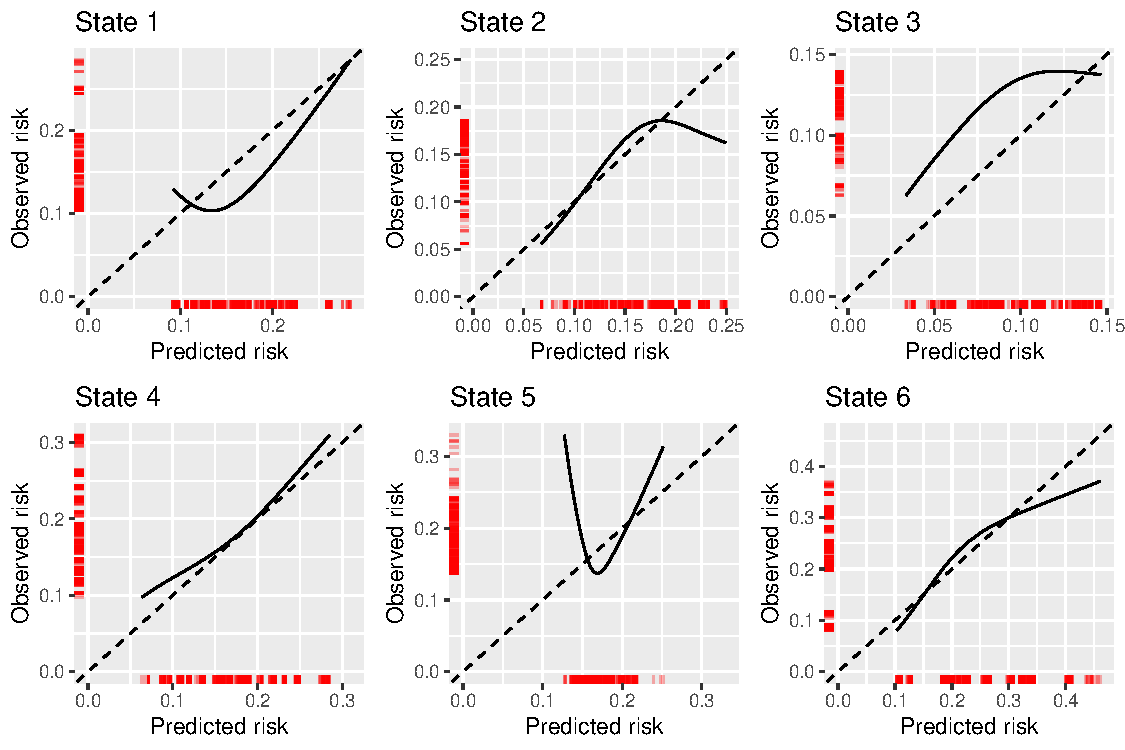
\includegraphics{overview-006}
\caption{\label{fig:blrj1s0} BLR-IPCW calibration curves out of state j =  1 at time s = 0.}
\end{figure}

Next we use the MLR-IPCW to evaluate calibration which produces a calibration scatter plot. The process is identical except the use of the function \code{calc_calib_mlr}. The MLR-IPCW calibration plots are contained in Figure \ref{fig:mlrj1s0}.

\begin{Schunk}
\begin{Sinput}
R> dat.calib.mlr <-
+    calc_calib_mlr(data.mstate = msebmtcal,
+                   data.raw = ebmtcal,
+                   j=1,
+                   s=0,
+                   t.eval = 1826,
+                   tp.pred = tps0 %>%
+                     dplyr::filter(j == 1) %>%
+                     dplyr::select(any_of(paste("pstate", 1:6, sep = ""))),
+                   w.covs = c("year", "agecl", "proph", "match"),
+                   w.landmark.type = "all")
\end{Sinput}
\end{Schunk}

\begin{figure}
\centering
\begin{Schunk}
\begin{Sinput}
R> plot(dat.calib.mlr, combine = TRUE)
\end{Sinput}
\end{Schunk}
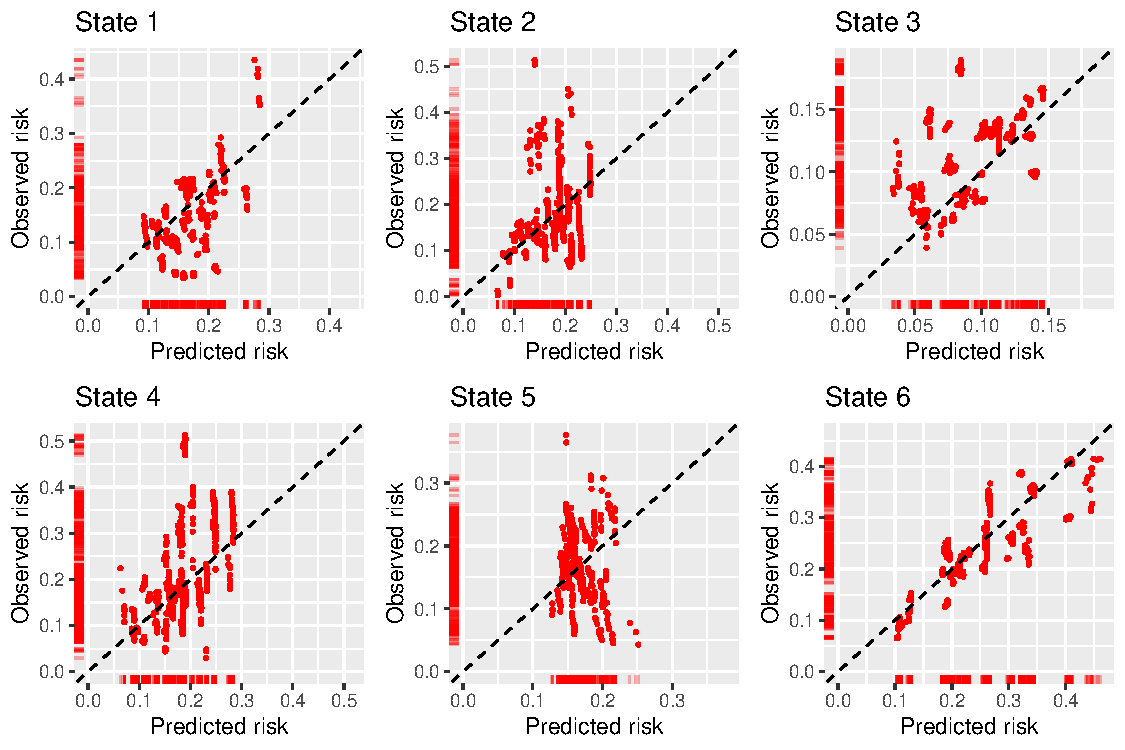
\includegraphics{overview-008}
\caption{\label{fig:mlrj1s0} MLR-IPCW calibration curves out of state j =  1 at time s = 0.}
\end{figure}

Within each plot for state $k$, there is a large amount of variation in calibration of the transition probabilities depending on the predicted transition probabilities into states $\neq k$. One valuable insight from these plots is that the variance in the calibration of the transition probabilities into state $6$, is smaller than that of state $4$, despite these two states both having similar (arguably state $4$ had better) calibration according to the BLR-IPCW plots. This insight can be gained because MLR-IPCW is a stronger form of calibration assessment than BLR-IPCW where calibration is being assessed within different levels of the predictor variables (which drive the predicted transition probabilities of all states). This type of calibration assessment also requires a bigger sample size as the confidence intervals around the observed event probabilities will be bigger than for BLR-IPCW. Furthermore, it is not clear how to present confidence intervals for all data points simultaneously. Given the relatively small number of data points we do not focus on the calibration scatter plots for the remainder of this example.

%% Subsection for s = 100
\subsection[Plots out of state j = 1 and 3 at time s = 100]{Plots out of state $j = 1$ and $3$ at time $s = 100$} \label{sec:plotss100}

In the work of \cite{DeWreede2011} focus then shifts to comparing transition probabilities when $s = 100$ depending on whether an individual has had an adverse event (state $3$) or remains in state $1$. Our focus now shifts to assessing the calibration of these transition probabilities. This is done using the landmarking approach described in section \ref{sec:methodology}. In \pkg{calibmsm}, the process remains the same, changing the inputted values \code{j} and \code{s}, and providing the appropriate predicted transition probabilities into the argument \code{tp.pred}. We start by producing the calibration plots for $j = 1$ and $s = 100$ (Figure \ref{fig:blrj1s100}).

\begin{Schunk}
\begin{Sinput}
R> dat.calib.blr.j1.s100 <-
+    calc_calib_blr(data.mstate = msebmtcal,
+                   data.raw = ebmtcal,
+                   j=1,
+                   s=100,
+                   t.eval = t.eval,
+                   tp.pred = tps100 %>%
+                     dplyr::filter(j == 1) %>%
+                     dplyr::select(any_of(paste("pstate", 1:6, sep = ""))),
+                   curve.type = "rcs",
+                   rcs.nk = 3,
+                   w.covs = c("year", "agecl", "proph", "match"))
\end{Sinput}
\end{Schunk}

\begin{figure}
\centering
\begin{Schunk}
\begin{Sinput}
R> plot(dat.calib.blr.j1.s100, combine = TRUE, nrow = 2, ncol = 2)
\end{Sinput}
\end{Schunk}
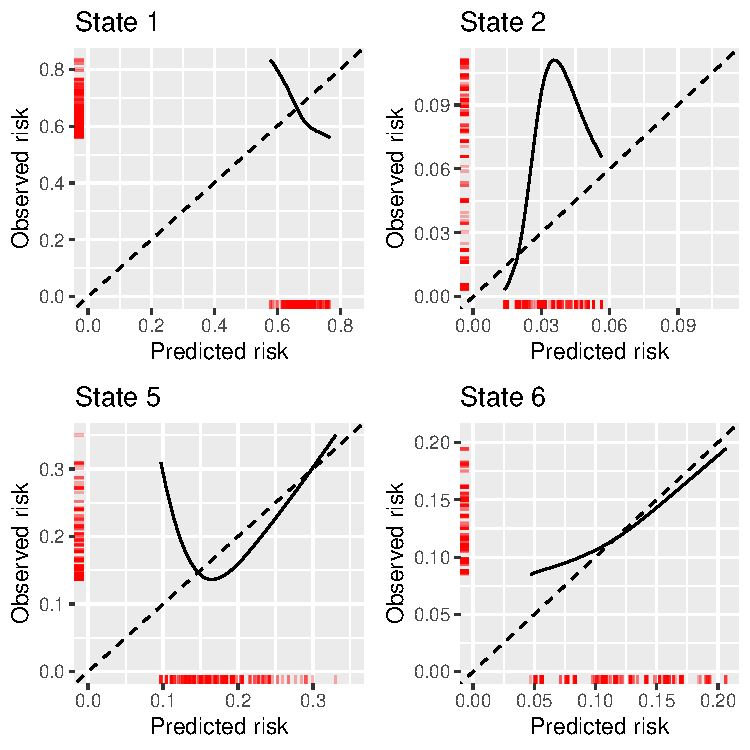
\includegraphics{overview-010}
\caption{\label{fig:blrj1s100} BLR-IPCW calibration curves out of state j =  1 at time s = 100.}
\end{figure}

There are only four calibration plots because no individuals in state $j = 1$ at time $s = 100$ are in states $3$ (adverse event) or $4$ (recovery + adverse event) after 1826 days. This is possibly due to the definition of an adverse event (must occur within a certain number of days after the transplant) \textbf{NOTE: I have scoured the internet but cannot confirm this, little information on the ebmt dataset used in this study. Should I remove this sentence, or leave?}. The calibration of the predicted transition probabilities are very poor. Only for state $6$ is the observed risk a monotonically increasing function of the predicted transition probability.

Next we produce calibration plots for $j = 3$ and $s = 100$ (Figure \ref{fig:blrj3s100}).

\begin{Schunk}
\begin{Sinput}
R> dat.calib.blr.j3.s100 <-
+    calc_calib_blr(data.mstate = msebmtcal,
+                   data.raw = ebmtcal,
+                   j=3,
+                   s=100,
+                   t.eval = t.eval,
+                   tp.pred = tps100 %>%
+                     dplyr::filter(j == 3) %>%
+                     dplyr::select(any_of(paste("pstate", 1:6, sep = ""))),
+                   curve.type = "rcs",
+                   rcs.nk = 3,
+                   w.covs = c("year", "agecl", "proph", "match"))
\end{Sinput}
\end{Schunk}

\begin{figure}
\centering
\begin{Schunk}
\begin{Sinput}
R> plot(dat.calib.blr.j3.s100, combine = TRUE, nrow = 2, ncol = 2)
\end{Sinput}
\end{Schunk}
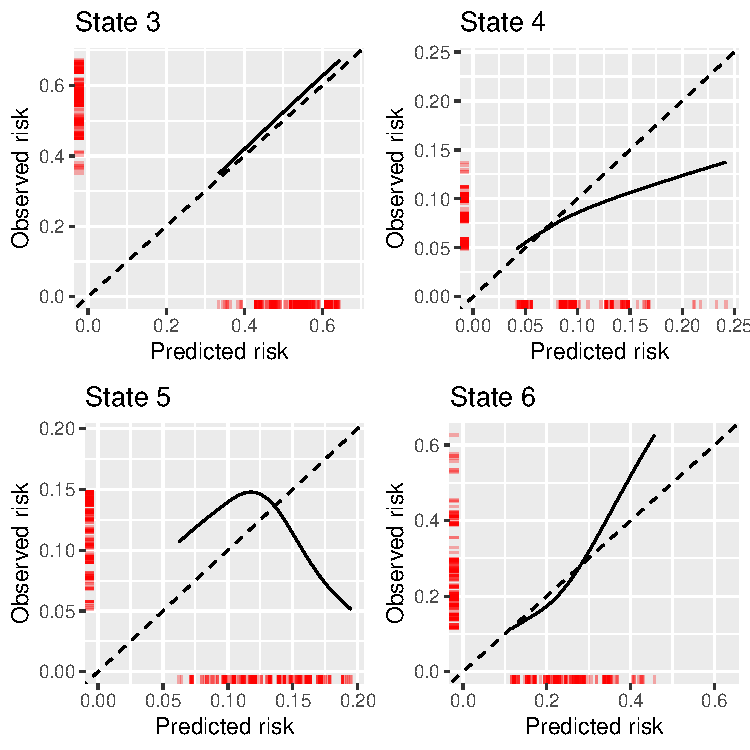
\includegraphics{overview-012}
\caption{\label{fig:blrj3s100} BLR-IPCW calibration curves out of state j =  3 at time s = 100.}
\end{figure}

Again there are only four possible states that an individual may transition into, although this includes states $3$ (adverse event) and $4$ (recovery + adverse event), instead of $1$ (transplant) and $2$ (recovery). In general the calibration plots are better than for $j = 1$, but large levels of miscalibration remain. Again the calibration of state $5$ is very poor, although the shape resembles a concave curve, rather than a convex one. This makes it difficult to base any clinical decisions on the predicted transition probabilities for relapse. On the contrary, the transition probabilities into death are reasonably well calibrated for both $j = 1$ and $j = 3$, (barring those with predicted risks bigger than $0.35$ for $j = 3$). This supports clinical decisions based on the risk of death after survival for 100 days.

So far all conclusions have been based on the estimated calibration curves, giving no thought to the variability with which these curves have been estimated. Estimation of the confidence interval around performance metrics is of paramount importance and the process for producing these is detailed in the next section.

%% Section 5 - confidence intervals
\section{Estimating confidence intervals for the calibration curves} \label{sec:calibci}

%% Subsection for calculating ci using internal procedure
\subsection{Estimating confidence intervals using internal bootstrapping procedure} \label{sec:internalci}

A process for estimating the confidence intervals around the calibration curves using bootstrapping has been built into the \code{calc_calib_blr} function. It goes:

\begin{enumerate}
 \item Resample validation dataset with replacement
 \item Calculate weights (note these may be calculated using either of the approaches outlined in section \ref{sec:weights} through the argument \code{w.landmark.type})
 \item Landmark the dataset for assessment of calibration
 \item Fit a calibration model in the landmarked dataset
 \item Generate observed event probabilities for a fixed vector of predicted transition probabilities (specifically the predicted transition probabilities from the non-bootstrapped landmark validation dataset)
\end{enumerate}

This will produce a number of bootstrapped calibration curves, all plotted over the same vectors of predicted transition probabilities. Taking the $\frac{\alpha}{2}$ and $\left(1-\frac{\alpha}{2}\right)$ percentiles of the observed event probabilities for each predicted transition probability gives the required $1-\alpha$ confidence interval around the estimated calibration curve. We reproduce Figure \ref{fig:blrj1s0} with the addition of a confidence interval estimated using the internal procedure. To enable this the size of the confidence interval \code{CI} and the number of bootstrap replicates \code{CI.R.boot} must be specified. A seed is also set for reproducibility.

\begin{Schunk}
\begin{Sinput}
R> set.seed(101)
R> dat.calib.blr <-
+    calc_calib_blr(data.mstate = msebmtcal,
+                   data.raw = ebmtcal,
+                   j=1,
+                   s=0,
+                   t.eval = t.eval,
+                   tp.pred = tps0 %>%
+                     dplyr::filter(j == 1) %>%
+                     dplyr::select(any_of(paste("pstate", 1:6, sep = ""))),
+                   curve.type = "rcs",
+                   rcs.nk = 3,
+                   w.covs = c("year", "agecl", "proph", "match"),
+                   CI = 95,
+                   CI.R.boot = 200)
\end{Sinput}
\end{Schunk}

\begin{figure}
\centering
\begin{Schunk}
\begin{Sinput}
R> plot(dat.calib.blr)
\end{Sinput}
\end{Schunk}
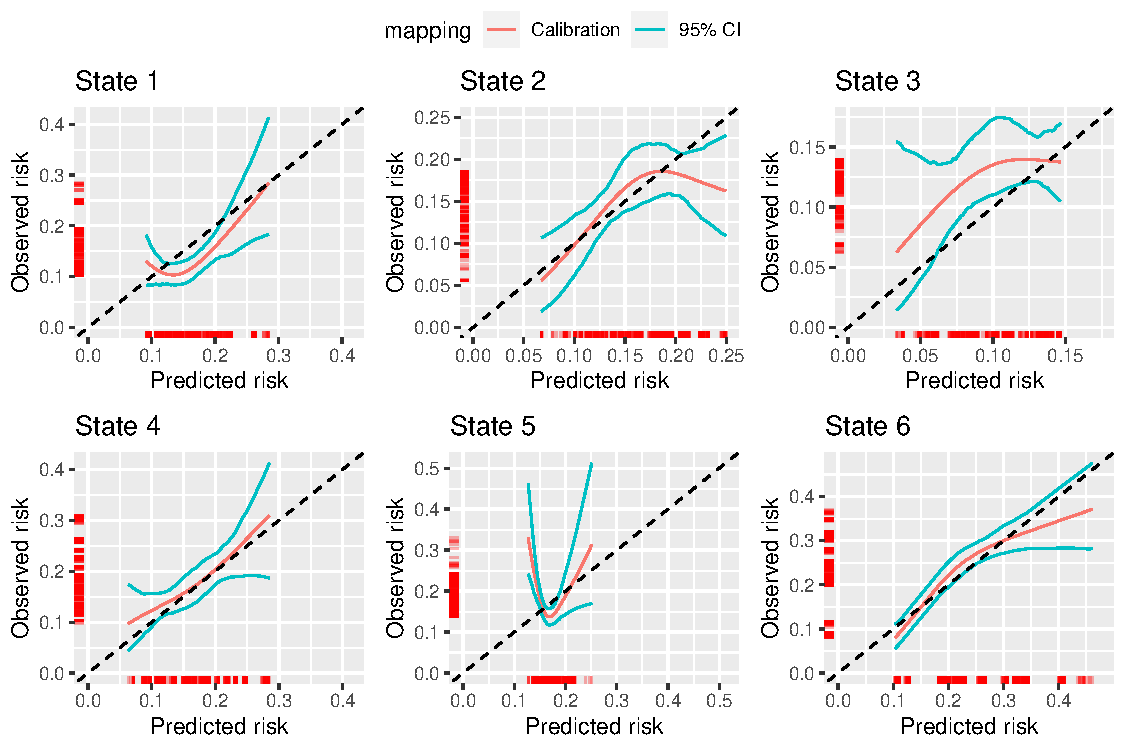
\includegraphics{overview-014}
\caption{\label{fig:blrj1s0ci} BLR-IPCW calibration curves out of state j =  1 at time s = 0 with confidence intervals estimated using internal procedure.}
\end{figure}

The calibration curves for the transition probabilities out of $j = 1$ at $s = 100$ are shown in Figure \ref{fig:blrj1s0ci}. The transition probabilities into states $k = 4$ and $6$ both contain the line of prefect calibration across the entire range of predicted risk. In the previous section, we discussed how for states $k = 4$ and $6$ calibration became imperfect for individuals with the lowest/highest predicted risks. These plots indicate this was possibly due to random variation, rather than biased estimation of the predicted transition probabilities, an issue that may be resolved by validating the model in a larger validation sample. On the contrary, we get confirmation that the calibration for transition probabilities into states $k = 1, 3$ and $5$ are miscalibrated over a large range of the predicted risks as the line of perfect calibration is outside of the confidence interval.

%% Subsection for calculating ci manually
\subsection{Estimating confidence interval manually using bootstrapping} \label{sec:manualci}

While the above approach is accessible, it may lead to a misspecified model for the  weights given the user has limited control over the functional form of the predictor variables $\textbf{Z}$. We encourage users to explore their data and produce a more suitable model to estimate the weights. Once estimated, these can be specified in the call to \code{calc_calib_blr} using the \code{weights} argument. To estimate the confidence interval the weights must be recalculated within each bootstrap sample. The \code{data.pred.plot} argument must be specified to ensure observed event probabilities are generated over the same vectors of predicted transition probabilities for each bootstrap sample, otherwise the confidence intervals cannot be plotted. For the remainder of this section, we demonstrate how to estimate a confidence interval for the calibration curve when estimating the weights manually. We follow the same five steps outlined at the start of section \ref{sec:internalci}. This is done in conjunction with the \pkg{boot} package \citep{Canty2022}.

We start by creating a permanent object with the predicted risks of each individual. When the validation cohort \code{ebmtcal} is resampled, the appropriate predicted transition probabilities must also be resampled from this object.

\begin{Schunk}
\begin{Sinput}
R> tp.pred <- tps0 %>%
+    dplyr::filter(j == 1) %>%
+    dplyr::select(any_of(paste("pstate", 1:6, sep = "")))
\end{Sinput}
\end{Schunk}

Next define the predicted transition probabilities over which the observed event probabilities will be plotted, which must be the same for every bootstrapped calibration curve. These are the predicted transition probabilities of the individuals who are uncensored at time \code{t.eval}, which are the predicted transition probabilities for the original calibration curves.

\begin{Schunk}
\begin{Sinput}
R> ## Extract ids for individuals uncensored at t.eval
R> ids.uncens <- ebmtcal %>%
+    subset(dtcens > t.eval | (dtcens < t.eval & dtcens.s == 0)) %>%
+    dplyr::pull(id)
R> ## Extract the predicted risks out of state 1 for these individuals
R> data.pred.plot <- tps0 %>%
+    dplyr::filter(j == 1 & id %in% ids.uncens) %>%
+    dplyr::select(any_of(paste("pstate", 1:6, sep = "")))
\end{Sinput}
\end{Schunk}

The calibration curves (with no confidence interval) are now calculated. We utilise the \code{calc_weights} function from \pkg{calibmsm} to estimate the weights, which is the function used internally. However, in practice the point of this exercise is to create a better performing model to estimate the weights than the one from the internal procedure. The vector of weights should have an entry for every row the validation dataset. For individuals who will not be included in the landmark cohort, or who are censored prior to time $t$, these weights can take any value as they will not be included when the calibration model is fitted.

\begin{Schunk}
\begin{Sinput}
R> weights.manual <-
+    calc_weights(data.mstate = msebmtcal,
+                 data.raw = ebmtcal,
+                 covs = c("year", "agecl", "proph", "match"),
+                 t.eval = t.eval,
+                 s = 0,
+                 landmark.type = "state",
+                 j = 1,
+                 max.weight = 10,
+                 stabilised = FALSE)$ipcw
R> str(weights.manual)
\end{Sinput}
\begin{Soutput}
 num [1:2279] NA 1.14 NA 1.01 1.03 ...
\end{Soutput}
\end{Schunk}

The observed event probabilities can then be estimated using \code{calc_calib_blr} and a call to the \code{weights} argument.

\begin{Schunk}
\begin{Sinput}
R> dat.calib.boot.manual <-
+    calc_calib_blr(data.mstate = msebmtcal,
+                   data.raw = ebmtcal,
+                   j=1,
+                   s=0,
+                   t.eval = t.eval,
+                   tp.pred = tp.pred,
+                   curve.type = "rcs",
+                   rcs.nk = 3,
+                   weights = weights.manual)
\end{Sinput}
\end{Schunk}

It is now time to estimate the confidence interval for this curve. We define a function \code{calc_obs_boot} to generate a bootstrapped calibration curve which is compatible with the \code{boot} function from the \pkg{boot} package. Within each bootstrapped dataset, weights are calculated and then a calibration curve is estimated using \code{calc_calib_blr}. The use of the argument \code{data.pred.plot} in \code{calc_calib_blr} is essential here, to ensure the bootstrapped observed event probabilities are generated for the same vectors of predicted transition probabilities. The function is also written to estimate a curve for the transition probabilities into a specific state $k$, as the output for \code{boot} must be a vector, rather than a matrix. This is done by utilising the \code{transitions.out} argument in \code{calc_calib_blr}.

\begin{Schunk}
\begin{Sinput}
R> calc_obs_boot <- function(data, indices, tp.pred, state.k){
+  
+    ## Bootstrap dataset and predicted transition probabilities
+    data.boot <- data[indices,]
+    tp.pred.boot <- tp.pred[indices, ]
+  
+    ## Calculate weights
+    ## In practice - replace this function with your own
+    weights.manual <-
+      calc_weights(data.mstate = msebmtcal,
+                   data.raw = data.boot,
+                   covs = c("year", "agecl", "proph", "match"),
+                   t.eval = t.eval,
+                   s = 0,
+                   landmark.type = "state",
+                   j = 1,
+                   max.weight = 10,
+                   stabilised = FALSE)$ipcw
+  
+    ## Estimate bootstrapped calibration curve
+    curve.est <-
+      calc_calib_blr(data.mstate = msebmtcal,
+                     data.raw = data.boot,
+                     j=1,
+                     s=0,
+                     t.eval = t.eval,
+                     tp.pred = tp.pred.boot,
+                     curve.type = "rcs",
+                     rcs.nk = 3,
+                     weights = weights.manual,
+                     data.pred.plot = data.pred.plot,
+                     transitions.out = state.k)
+  
+    ## Extract observed event probabilities
+    curve.obs <-
+      curve.est[["plotdata"]][[paste("state", state.k, sep = "")]]$obs
+  
+    return(curve.obs)
+  
+  }
\end{Sinput}
\end{Schunk}

The size of the confidence interval, the states $k$ which individuals may transition into from state $j$, and a list to store the data for the plots are then defined:

\begin{Schunk}
\begin{Sinput}
R> alpha <- (1-95/100)/2
R> valid.transitions <- which(colSums(tp.pred) != 0)
R> plot.data.list <- vector("list", length(valid.transitions))
\end{Sinput}
\end{Schunk}

The bootstrap procedure is now applied to the validation dataset \code{ebmtcal} for each state $k$ in \code{valid.transitions}, and the upper and lower confidence bands are stored in a \code{data.frame} along with the calibration curve calculated earlier.

\begin{Schunk}
\begin{Sinput}
R> for (k in 1:length(valid.transitions)){
+  
+    ## Assign state k
+    state.k <- valid.transitions[k]
+  
+    ## Run bootstrapping
+    boot.obs <- boot::boot(ebmtcal,
+                           calc_obs_boot,
+                           R = 200,
+                           tp.pred = tp.pred,
+                           state.k = state.k)$t
+  
+    ## Extract confidence bands
+    lower <- apply(boot.obs, 2, stats::quantile, probs = alpha, na.rm = TRUE)
+    upper <- apply(boot.obs, 2, stats::quantile, probs = 1-alpha, na.rm = TRUE)
+  
+    ## Assign output
+    plot.data.list[[k]] <- data.frame(
+      "pred" = dat.calib.boot.manual[["plotdata"]][[k]]$pred,
+      "obs" = dat.calib.boot.manual[["plotdata"]][[k]]$obs,
+      "obs.lower" = lower,
+      "obs.upper" = upper)
+  
+  }
\end{Sinput}
\end{Schunk}

Finally, metadata is added and the appropriate \code{class} is defined so that the data is in the same format as the output from \code{calc_calib_blr}, meaning it can be used with the S3 generic \code{plot}.

\begin{Schunk}
\begin{Sinput}
R> metadata <- list("valid.transitions"= valid.transitions,
+                   "CI" = 95,
+                   "curve.type" = "rcs")
R> dat.calib.blr.manual <- list("plotdata" = plot.data.list, "metadata" = metadata)
R> attr(dat.calib.blr.manual, "class") <- "calib_blr"
\end{Sinput}
\end{Schunk}

The calibration curves with manually estimated confidence intervals are plotted in Figure \ref{fig:blrj1s0cimanual}. This Figure is very similar to Figure \ref{fig:blrj1s0ci}. This is to be expected given we have used the same model to estimate the weights that is used in the internal procedure, and verifies that the manual procedure for calculating the confidence interval has been successful.

\begin{figure}
\centering
\begin{Schunk}
\begin{Sinput}
R> plot(dat.calib.blr.manual)
\end{Sinput}
\end{Schunk}
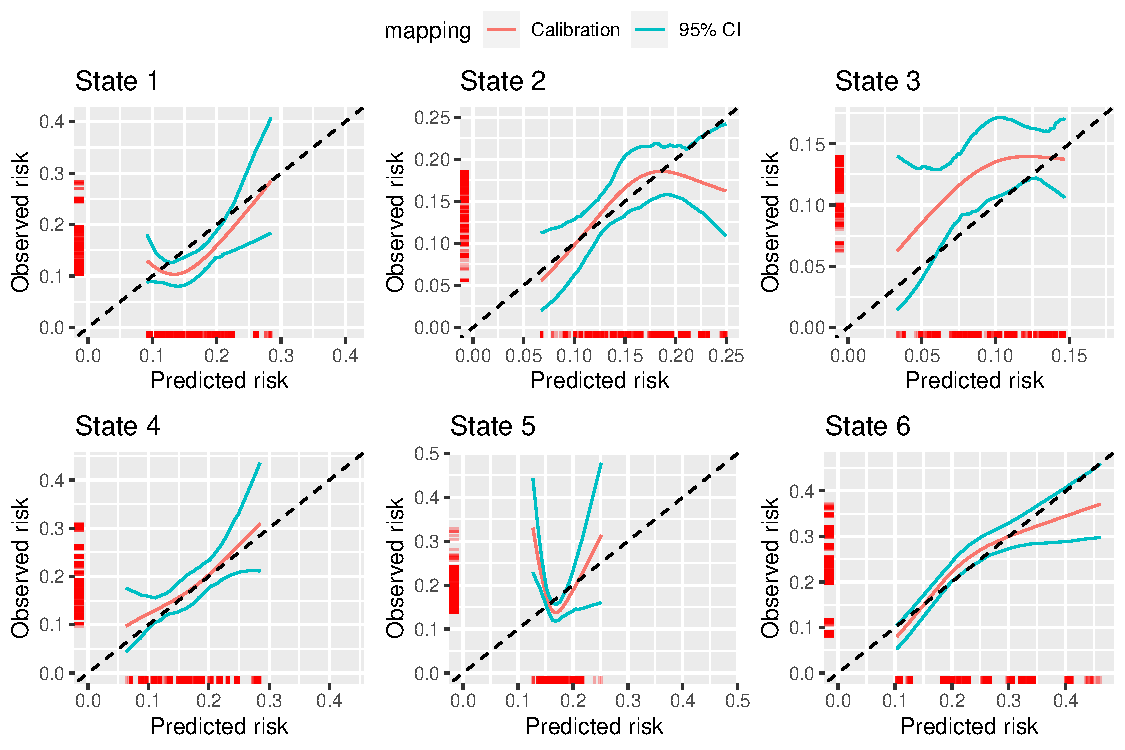
\includegraphics{overview-023}
\caption{\label{fig:blrj1s0cimanual} BLR-IPCW calibration curves out of state j =  1 at time s = 0 with confidence intervals estimated manually using bootstrapping.}
\end{figure}

%% Section 6 - Discussion

\section{Discussion} \label{sec:discussion}

Multistate models are a useful and unique tool for prediction, allowing risks to be updated after key events happen post baseline. Development of multistate models for prediction is becoming more common, yet validation of such models is still very uncommon. A major barrier to implementation of statistical techniques is often the availability of software \citep{Pullenayegum2016}. \pkg{calibmsm} has been developed to aid in the implementation of techniques to assess the calibration of transition probabilities from a multistate model. This paper has extended a previously proposed framework for assessing the calibration of the transition probabilities out of the initial state \textbf{XXXX REF project 6 (probably have to put on Arxiv)}, to the transition probabilities out of any state $j$ at any time $s$.

The BLR-IPCW and MLR-IPCW methods have been shown to give an unbiased assessment of calibration under non-informative censoring mechanisms, and a predominately unbiased assessment of calibration under strongly informative censoring \textbf{XXXX REF PROJECT 6}. Despite this, further research evaluating these methods performance in a wider range of simulation scenarios, and by a different research group \citep{Boulesteix2013}, would be highly valuable \citep{Heinze2022}. Further to this point, it is possible to use the \pkg{calibmsm} to validate competing risks models, which are a special case of a multistate models. However, graphical calibration curves already exist for assessing the calibration of a competing risks model \citep{Austin2022}. When fitting graphical calibration curves, it is assumed that censoring is independent of the outcome after conditioning on the complementary log-log transformation of the predicted risk, and the assumption of proportional hazards is made. When implementing BLR-IPCW, the assumption of independence between the censoring mechanism and the outcome in the reweighted population is made. These are different approaches to dealing with the same problem. Graphical calibration curves have the advantage that only one model needs to be fit and calibration can be assessed at every possible follow up time $t$. Beyond this, it is unclear in what scenarios each approach is preferable. Simulations comparing these approaches when the aforementioned assumptions do and do not hold would be valuable. Both of these suggestions would constitute phase 3 and 4 studies in the evidence base for new methods \citep{Heinze2022}. Such simulations should be made easier by the existence of \pkg{calibmsm} to implement BLR-IPCW and MLR-IPCW.

\textbf{I have not done the following sensitivity analyses yet, these are just my suggestions.}

We have ran a series of sensitivity analyses in this study which are presented in the supplementary material. First, we produced equivalent calibration plots for each Figure using pseudo-values based on the Aalen-Johansen estimator. This approach was found to have similar performance to BLR-IPCW \textbf{XXXX REF PROJECT 6}. This method has not been included in \pkg{calibmsm} due to the computational time taken to apply this method. Agreement between the calibration plots would provide some validation to the results produced by BLR-IPCW. We wanted to measure its performance closely due to reliance on correct estimation of the weights. Second, we compared the calibration curves of BLR-IPCW with the graphical calibration curves and found.... \textbf{note to self} Thirdly, I want to do some validation of the stabalised weights. This will probably not be included in the paper, something I want to do to verify behaviour is as expected.

%% -- Optional special unnumbered sections -------------------------------------
\section*{TO DO}

\begin{enumerate}
  \item Check the rug plots are being implemented with transparency, and add a input parameter to change the transparency
  \item Check the MLR-IPCW plots are being implemented with transparency, and add a input parameter to change the transparency
  \item Add some proper warnings into the functions in the package for stuff I have listed somewhere
\end{enumerate}

\section*{Computational details}

\textbf{WILL UPDATE THIS SECTION ONCE PACKAGE HAS BEEN FINALISED AND UPLOADED TO CRAN}

The results in this paper were obtained using
\proglang{R}~4.3.0 with the
\pkg{dplyr}~1.1.2,
\pkg{tidyr}~1.3.0,
\pkg{ggplot2}~3.4.2,
\pkg{ggpubr}~0.6.0,
\pkg{Hmisc}~5.0.1,
\pkg{rms}~6.6.0,
\pkg{VGAM}~1.1.8,
\pkg{boot}~1.3.28.1,
\pkg{survival}~3.5.5,
\pkg{stats}~4.3.0,
\pkg{magrittr}~2.0.3. \proglang{R} itself
and all packages used are available from the Comprehensive
\proglang{R} Archive Network (CRAN) at
\url{https://CRAN.R-project.org/}.

\section*{Acknowledgments}

\begin{leftbar}
Thank you to Thomas Yee for helping to debug an issue with implementing vector spline smoothers from the \pkg{VGAM} package within \pkg{calibmsm}.
\end{leftbar}

\bibliography{refs}

%% -- Appendix (if any) --------------------------------------------------------
%% - After the bibliography with page break.
%% - With proper section titles and _not_ just "Appendix".

\newpage

\begin{appendix}

\section[Comparison of calibration curves for transition probabilities generated using pseudo-values]{\texorpdfstring{Comparison of calibration curves for transition probabilities generated\\ using pseudo-values}{Comparison of calibration curves for transition probabilities generated using pseudo-values}} \label{app:pseudo}

\section[Comparison of BLR-IPCW calibration curves for competing risks sub-models with those generated using graphical calibration curves]{\texorpdfstring{Comparison of BLR-IPCW calibration curves for competing risks sub-models with those generated using graphical calibration curves}{Comparison of BLR-IPCW calibration curves for competing risks\\ sub-models with those generated using graphical calibration curves}} \label{app:gcc}

% \begin{leftbar}
% Appendices can be included after the bibliography (with a page break). Each
% section within the appendix should have a proper section title (rather than
% just \emph{Appendix}).
%
% For more technical style details, please check out JSS's style FAQ at
% \url{https://www.jstatsoft.org/pages/view/style#frequently-asked-questions}
% which includes the following topics:
% \begin{itemize}
%   \item Title vs.\ sentence case.
%   \item Graphics formatting.
%   \item Naming conventions.
%   \item Turning JSS manuscripts into \proglang{R} package vignettes.
%   \item Trouble shooting.
%   \item Many other potentially helpful details\dots
% \end{itemize}
% \end{leftbar}
%
%
% \section[Using BibTeX]{Using \textsc{Bib}{\TeX}} \label{app:bibtex}
%
% \begin{leftbar}
% References need to be provided in a \textsc{Bib}{\TeX} file (\code{.bib}). All
% references should be made with \verb|\cite|, \verb|\citet|, \verb|\citep|,
% \verb|\citealp| etc.\ (and never hard-coded). This commands yield different
% formats of author-year citations and allow to include additional details (e.g.,
% pages, chapters, \dots) in brackets. In case you are not familiar with these
% commands see the JSS style FAQ for details.
%
% Cleaning up \textsc{Bib}{\TeX} files is a somewhat tedious task -- especially
% when acquiring the entries automatically from mixed online sources. However,
% it is important that informations are complete and presented in a consistent
% style to avoid confusions. JSS requires the following format.
% \begin{itemize}
%   \item JSS-specific markup (\verb|\proglang|, \verb|\pkg|, \verb|\code|) should
%     be used in the references.
%   \item Titles should be in title case.
%   \item Journal titles should not be abbreviated and in title case.
%   \item DOIs should be included where available.
%   \item Software should be properly cited as well. For \proglang{R} packages
%     \code{citation("pkgname")} typically provides a good starting point.
% \end{itemize}
% \end{leftbar}
%
\end{appendix}

%% -----------------------------------------------------------------------------


\end{document}
